\subsection{The coverage definition changes the selected rule}
\label{sec:policy-choice}
\begin{table}[t]
\centering\small
\caption{Coverage changes the selected rule. Thresholds and the case/exposure choices use calibration outcomes only. Differences are exposure-choice minus case-choice on evaluation data (percentage points). Intervals are paired cluster-bootstrap 99.375\% intervals, adjusted across the eight primary coverage contrasts; all eight exclude zero. These additional menu comparisons are retrospective.}
\label{tab:policy-choice}
\begin{tabular}{llrr}
\toprule
Setting & Selected by cases / exposure & $\Delta c$ & $\Delta d$ [adjusted interval] \\
\midrule
M5: L1 & Excess / Exposure descending & -40.66 & 7.64 [4.24, 11.97] \\
M5: residual & Excess / Exposure descending & -35.18 & 8.31 [5.47, 11.69] \\
M5: Chronos-2 & Excess / Exposure descending & -39.61 & 10.63 [7.37, 14.49] \\
Bike Sharing & Excess / Ratio & -13.34 & 5.01 [1.93, 8.56] \\
\bottomrule
\end{tabular}
\end{table}

Case coverage chooses the excess ranking for all four primary menus. Exposure coverage chooses descending predicted demand for all three retail predictors and the fitted ratio for Bike. Thus the practical implication is not to prescribe one score everywhere: the utility determines which candidate to select, and the empirical winner depends on the task.

These calibration choices retain their coverage contrast on evaluation data (Table~\ref{tab:policy-choice}). For the residual predictor, changing the selected rule raises covered demand from 83.85\% to 92.15\% while reducing accepted cases from 89.50\% to 54.32\%. All eight adjusted coverage intervals exclude zero. The three retail comparisons share items, and this additional analysis is retrospective. It measures the consequence of selecting among these five rules, not a general benchmark ranking of uncertainty estimators.

\begin{figure}[t]
\centering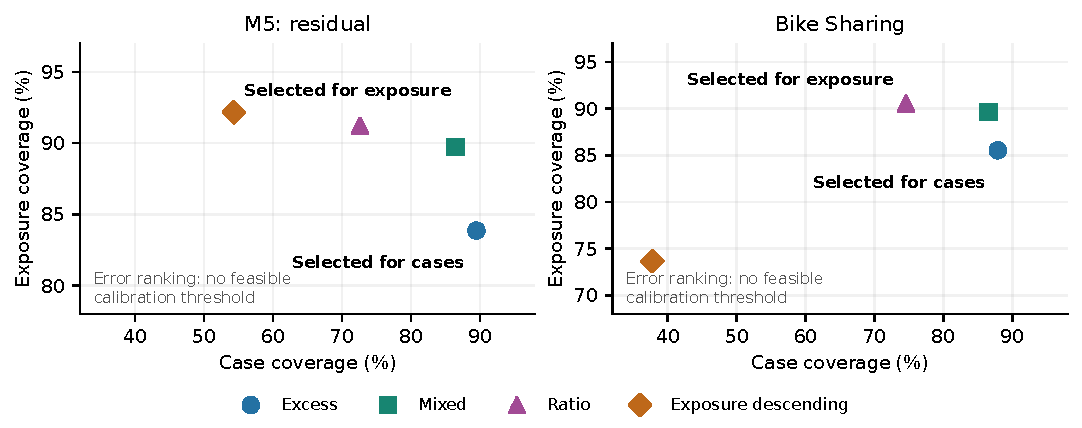
\includegraphics[width=\linewidth]{figures/policy_choice.pdf}
\caption{One predictor and one calibration-feasible candidate menu per panel. Labels identify rules selected by calibration utility; coordinates are evaluation coverages. The exposure choice is the simple descending-exposure baseline on M5 and the ratio on Bike. No line is drawn as a Pareto frontier. Point-risk feasibility does not imply a certified risk bound.}
\label{fig:policy-choice}
\end{figure}

The cap sweep also changes the exposure-selected family: the fitted ratio is selected at stricter retail caps, whereas descending predicted exposure is selected at the original cap. At a sufficiently loose cap both choices accept all and the contrast vanishes. The conditional-error ranking has no feasible threshold at the primary caps under the stated floor. Every declared cap is retained in Appendix Table~\ref{tab:choice-caps}. At .68 only the residual predictor has zero contrast; L1 and Chronos retain it. Cap dependence is part of the result, not evidence for a universally preferred cap or score.

